%%
%% This is file `example/ch_concln.tex'
%% generated with the docstrip utility.
%%
%% The original source files were:
%%
%% install/buptgraduatethesis.dtx  (with options: `ch-concln')
%% 
%% This file is a part of the example of BUPTGraduateThesis.
%% 

\chapter{相关技术概述}
SDN作为新一代的网络架构,具有动态配置、可编程及快速响应的特点,通过控制平面与数据转发平面的分离,实现了对底层网络基础设施的抽象。OpenStack作为当下最流行的开源云平台之一,主要为用户提供计算、存储、网络等服务。本章对SDN、OpenFlow、OpenStack等相关技术做了详细的介绍。
\section{SDN、OpenFlow概述}
\subsection{SDN简介}
SDN是一种时下热门的网络架构,在这种网络架构中,网络的控制与转发解耦,具有很强的可扩展性和可编程性。传统模式下,网络的控制权与网络设备紧密捆绑,现有模式下,控制权的迁移使得底层构架能够抽象出来,各种网络服务及应用因此可以将网络当作一个虚拟实体。通过应用SDN,网络设备得到简化,这些设备在SDN模式下无需识别或处理成千上万种协议,只需要接受SDN 控制器的管控即可。集中控制的实现,使得网络管理员可以实时改变网络行为,并且在几小时或几天内实现新应用和网络服务的部署工作\cite{SDN-3}。

\begin{figure}[!htb]
  \centering
  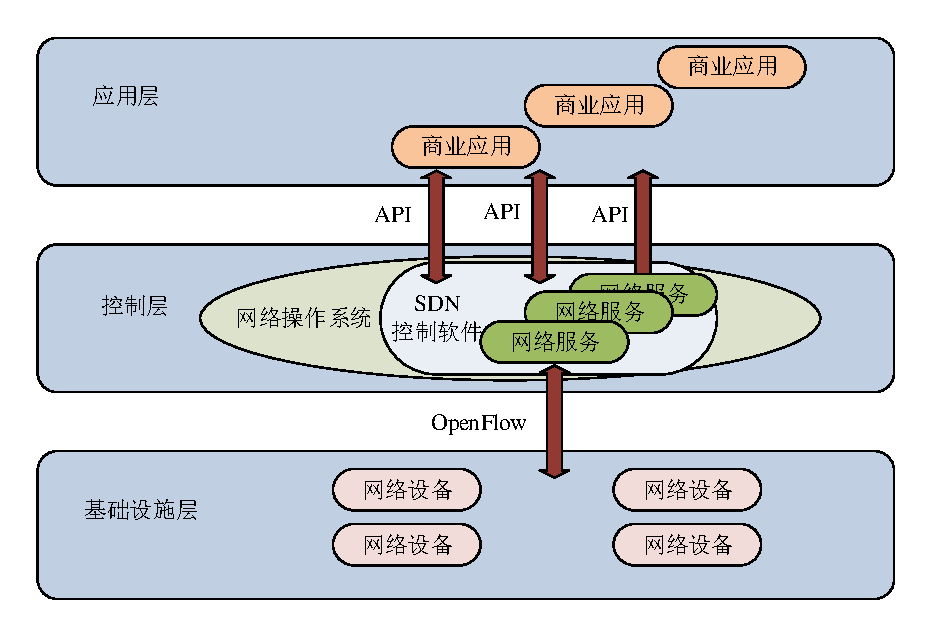
\includegraphics[width=0.7\textwidth]{logo/sdn}
  \caption{ONF定义的SDN三层架构图}
  \label{fig:sdn}
\end{figure}

现有 SDN 体系由应用层、控制层和转发层构成。详细架构图如图\ref{fig:sdn}所示\cite{SDN-2}。

应用层主要为网络提供各种网络应用需求,通过北向接口,灵活地调用控制层提供的可编程的业务功能。控制层是整个SDN构架的核心部分,其主要功能包括网络的虚拟化、网络拓扑管理、路由策略优化等,控制层的分离,实现了对网络更为灵活的管控。基础设施层包括标准化的网络设备和虚拟的网络设备,负责多级流表处理和高性能的数据转发,并作为硬件资源池,为控制层提供按需的网络拓扑、数据处理和数据转发。南向接口定义了控制层与基础设施层之间的协议标准,底层的物理设备被抽象为资源池,控制器通过将数据包的转发过程抽象为流表的下发过程,实现了对流表的直接控制,屏蔽了与硬件设备的兼容性问题,截止到目前,控制器与数据转发层之间最主流的交互协议为OpenFlow协议\cite{openflow-9}。
\subsection{OpenFlow协议}
OpenFlow协议是OpenFlow交换机与控制器之间进行信息交互的标准,OpenFlow协议主要包含三种类型的消息,分别为Controller-to-Switch消息,Asynchronous 消息以及Symmetric 消息。Controller-to-Switch消息由控制器传递给交换机,主要实现控制器对交换机的监视和管理工作,必要情况下需要交换机对接收到的消息做出回应;Asynchronous消息是由交换机发送给控制器,主要用于更新交换机自身的状态,同时将该状态变更传递给控制器;Symmetric消息可以由交换机或者控制器任意一方发起\cite{openflow-5}。对于每种消息都具有多个子类型,具体协议子类型及其描述如下所示。

\begin{enumerate}
\item Controller-to-Switch消息
\begin{itemize}
\item Features:该消息用于建立传输层安全会话(Transport Layer Security Session)时使用,由控制器发送该消息至交换机,交换机需要做出应答。一般在 OpenFlow 安全通道建立的时候使用。
\item Configuration:用于控制器对交换机配置信息的设置和查询。交换机查询相应的配置信息,将查询结果回复给控制器。
\item Modify-state:用于控制器对交换机流表以及端口状态的管理更新。
\item Read-state:控制器使用该消息向交换机请求网络统计信息,比如网包、流等。
\item Packet-out:该消息由控制器发送给交换机,通过指定的交换机端口发送该网包。该消息必须包含一个完整的网络数据包,或者包含网包的部分内容以及网包在交换机缓存中存储的ID号。 
\end{itemize}
\item Asynchronous消息
\begin{itemize}
\item Packet-in:该消息由交换机触发,发送给控制器端,当数据包到达交换机,交换机中不存在匹配的流表项时,交换机会触发该消息,发送给控制器,控制器解析该消息,通过全局的网络拓扑查询转发链路,下发流表,实现数据包的转发工作。交换机可以将数据包全部发送给控制器,亦可将数据包存储在交换机缓存中,仅仅将数据包的部分内容和交换机缓存ID号发送给控制器。具体视交换机的缓存大小而定。
\item Flow-removed:该消息用于交换机中流表项的删除工作
\item Port-status:更新交换机端口状态。
\item Error:交换机异常时触发。
\end{itemize}
\item Symmetric消息
\begin{itemize}
\item Hello:该消息用于控制器和交换机之间连接的建立。
\item Echo:该消息主要用于带宽、时延的测量以及控制器与交换机连接状态的获取。
\item Vendor:该消息为未来版本预留,现阶段不起任何作用,未来主要为交换机提供额外功能。
\end{itemize}
\end{enumerate}

OpenFlow协议的主要交互过程如下所示:

\begin{enumerate}
\item 控制器与交换机建立连接:通过安全通道,实现控制器和交换机连接的建立,在连接建立以后,某一方发送OFPT\_HELLO消息,该消息中包含本方所支持的OpenFlow协议的最高版本号,接收方,使用双方均支持的OpenFlow协议的最低版本进行通信传输。如果两者没有均支持的版本号,则连接建立失败。
\item 控制器与交换机连接中断:当控制器与交换机的连接发生异常时,交换机会断开与主控制器建立的连接,转而尝试与备用控制器建立连接,当多次尝试仍无法实现连接建立时,交换机便进入紧急模式,此时,交换机对接收到的数据包全部匹配紧急模式流表进行转发,对于普通的流表项,会从交换机中删除。默认在交换机启动时,进入紧急模式状态。
\item 连接加密:交换机与控制器建立连接的过程需要经过安全通道,安全通道采用\gls*{TLS}协议进行连接加密。在每个交换机启动的时候,会尝试与控制器建立连接,双方通过交换各自的证书进行认证,认证成功后,方能实现连接的建立。
\item 流表项修改:该过程为SDN模式下的核心交互过程,通过控制器下发流表修改的指令,实现交换机对流表项的删除、增加和修改工作。
\item 流表项的移除包含两种模式,分别为控制器主动模式和被动模式。控制器主动模式下,控制器通过主动下发 DELETE指令,实现对交换机中流表项的删除;而对于被动模式,每条交换机流表中包含超时属性,超时属性由定时器计时实现,主要记录流表距离上次匹配的时间,以及流表的存活总时间,当某条流表存活时间超过该限制时,交换机将自动删除该流表项,同时告知控制器。
\end{enumerate}

\subsection{OpenFlow交换机}
OpenFlow交换机主要负责数据的转发功能,其架构由流表(flow table)、安全信道(secure channel)组成\cite{openflow-1},OpenFlow交换机架构图如图\ref{fig:of-switch}所示。

\begin{figure}[!htb]
  \centering
  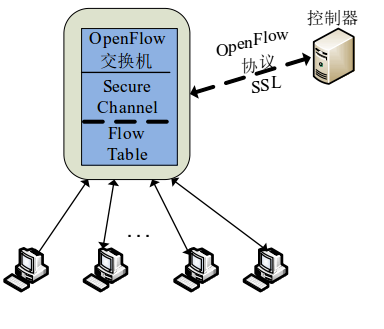
\includegraphics[width=0.7\textwidth]{logo/of-switch}
  \caption{OpenFlow交换机结构}
  \label{fig:of-switch}
\end{figure}

OpenFlow交换机中针对数据包的转发策略全部保存在流表信息中,每个流表都由很多表项组成,最终实现数据包的匹配和转发工作。这些表项的属性值均由控制器实现写入、更新和删除。现阶段,OpenFlow协议已由1.0版本发展至1.4版本,本文针对OpenFlow\ v1.3进行讲解,该版本中,每条流表均由匹配域、优先级、计数器、指令、超时以及Cookie组成\cite{openflow-8},具体如表\ref{table:flow}所示。当交换机接收到数据包时,会按照匹配域进行流表匹配,按照匹配上的流表,执行相应的转发动作。当同时匹配上多个流表时,按照优先级最高的流表项的指令进行转发。与此同时,更新流表中计数器、超时等属性值。

\newcommand{\enter}[2][c]{%
  \begin{tabular}[#1]{@{}c@{}}#2\end{tabular}}
\begin{table}[!htb]
    \centering
	\caption{OpenFlow流表项结构}
	\label{table:flow}
	\begin{tabular}{|c|c|c|c|c|c|}
	\hline 
	\enter{匹配域 \\(Match Field)}& \enter{优先级 \\(Priority)}& \enter{计数器 \\(Counters)}& \enter{指令\\(Instructions)}&\enter{超时 \\(Timeouts)} & Cookie \\
	\hline
	\end{tabular}
\end{table}

OpenFlow流表项的详细介绍如下所示。

\begin{itemize}
  \item 匹配域:用于实现对流的匹配工作,主要包含13个匹配域,分别为:以太网源地址、目的地址,交换机入端口,IP协议号、流的类型,IPv4的源地址、目的地址,IPv6的源地址、目的地址,TCP的源端口、目的端口号,UDP的源端口、目的端口号。对于每一个域,都会有一个确定的值用于对流进行匹配,如果该值设为Any,表示匹配任意一个流。
  \item 优先级:当交换机针对某个数据包匹配到多个流表项时,交换机会选取优先级最高的流表为匹配流表,执行该条流表的指令,完成数据包的转发。
  \item 计数器:主要用于统计每条流表的信息,主要包括该条流表被匹配的次数、发送包匹配数、接收包匹配数、发送字节匹配数以及接收字节匹配数。当数据包匹配上某条流表时,在执行完该条流表的指令后,流表相应地更新计数器各属性值。
  \item 超时:主要用于自动删除交换机中超时的流表。由于交换机中存储流表的数量是有限的,该超时机制的存在,可以在很大程度上提高交换机的空间利用率。
\end{itemize}

在数据包到达交换机后,交换机会根据数据包携带的信息进行流表的匹配工作,匹配的具体过程如图\ref{fig:match}所示,具体流程如下。

\begin{enumerate}
\item 从数据包中提取其匹配信息,根据匹配信息的字段名和属性值,进行流表的匹配工作。首先需要获取匹配信息的字段名,通常情况下,该字段名来自于数据包的报头,主要包括IP源地址或目的地址、以太网源地址或目的地址,当然也可以是数据包的入端口或出端口。 
\item 从数据包中提取出匹配字段的值,在交换机流表中查找匹配项。如果某条流表中的字段具有该属性值,就实现了数据包的匹配工作,如果存在多条流表同时匹配上该数据包,选取优先级最高的流表进行匹配,此时按照匹配流表的指令执行相应的操作。如果该数据包未匹配上流表,交换机会转发该数据包给控制器,通过控制器进行流表下发,实现相应的转发工作\cite{openflow-7}。
\end{enumerate}

\begin{figure}[!htb]
  \centering
  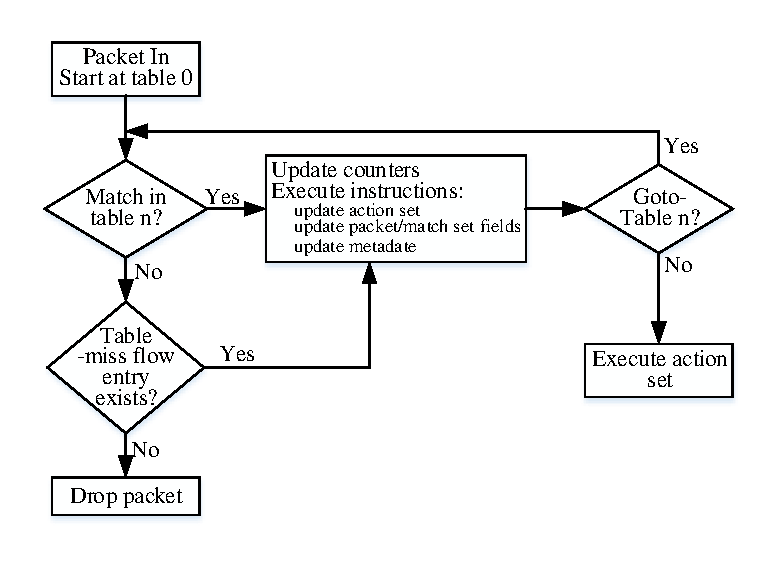
\includegraphics[width=0.7\textwidth]{logo/match}
  \caption{数据包匹配流程图}
  \label{fig:match}
\end{figure}

安全通道用于连接SDN控制器和OpenFlow交换机,控制器通过安全通道与交换机建立连接,实现对OpenFlow交换机的集中管控。与此同时,交换机亦通过该通道将消息上传给控制器。所有经安全通道传输的信息必须经由OpenFlow协议进行封装,OpenFlow安全通道通常用TLS进行加密,保证信息传输的安全性。

现阶段,主要存在两个版本的软件OpenFlow交换机\cite{openflow-2},分别为:基于用户空间的OpenFlow交换机和基于内核空间的OpenFlow交换机。前者使用简单,便于用户进行修改操作,缺点是性能相对较差;而后者速度较快,同时可以通过虚拟化技术,使得用户的虚拟机可以通过虚拟网络进行数据传输,缺点是用户的修改操作相对较复杂\cite{openflow-3}。对于硬件交换机,斯坦福大学实现了基于 NetFPGA的硬件加速OpenFlow交换机\cite{openflow-4},NEC、HP 等公司也相继推出了支持 OpenFlow 协议的硬件交换机\cite{openflow-1}。
\subsection{OpenFlow控制器}
控制器作为OpenFlow网络的核心部分,是整个网络的操作系统,网络中所有控制指令的下发,数据流转发策略的制定都由它来完成,控制器中组件的好坏直接影响了整个网络的运行效率。

SDN南向接口,主要实现了SDN控制器对底层网络的集中控制,控制器通过南向接口协议,可以进行流表下发、策略制定、链路探测、拓扑管理等功能。对于流表下发以及策略制定,控制器通过南向接口的下行通道,下发流表,实现对底层设备的集中管控。对于拓扑管理和链路探测,交换机通过南向接口上报网络信息实现。在数据流处理的过程中,控制器的控制程序决定其所在网络中交换机上的流表内容。在网路初始运行时,交换机上的流表均为空,控制器根据当前网络运行状态以及拓扑信息,针对不同数据流做出正确的决策。

SDN北向接口主要为上层应用提供开放的可编程接口\cite{SDN-4},用户通过该接口实现对底层网络资源的灵活调用。与此同时,用户通过控制器的北向接口,开发定制化应用,满足特定的网络需求。由于北向接口是面向应用层,北向接口设计的合理性、便捷性,很大程度上影响到SDN控制器的市场前景。

SDN控制器作为网络的操作系统,集中控制整个SDN网络。控制能力的集中化,使得控制器的性能成为SDN网络的瓶颈,因此如何保证SDN控制器的高可靠性成为开发者的研究重点之一,针对单节点的控制层,较常见的方案是构建主备模式的控制器架构,在主控制器出现异常时,底层网络自动切换至备用控制器,由备用控制器实现对网络的集中化管控。

\section{网络虚拟化技术概述}
随着互联网的飞速发展,必然会出现越来越多的应用和服务,现有相对固化的网络架构,可扩展性极低,而研发新的网络体系架构较困难,无法在短时间内保证网络架构的成熟稳定,并且现有的网络设备生产厂商均追求自身利益,更加剧了这些困难。在这种背景下,网络虚拟化成为向未来网络体系架构过渡的关键技术之一。

网络虚拟化技术\cite{Virtual-1},通过对物理基础设施资源进行抽象,并为用户提供统一的北向可编程接口,将多个相互隔离的租户虚拟网络映射到底层同一物理网络上,为用户提供差异化的服务。传统的网络虚拟化配置和操作都比较复杂,难以管理,原因是路由器和交换机变的越来越复杂,随着集群规模的增大,配置操作的成本越来越大。而在SDN架构下,网络虚拟化的实现变得容易很多,在SDN网络中,控制器的集中控制使得对网络的管理变得灵活、高效。

本文选用OVX实现网络虚拟化模块,OVX通过给每个租户提供一个可以访问的虚拟网络拓扑和一个完整的网络头空间来实现网络的虚拟化,前者可以实现租户对虚拟网络拓扑的自定义,而后者实现了租户之间的流量隔离,并且不同租户可以共用相同的寻址方案,即不同租户虚拟机可以使用相同的虚拟IP。OVX用作控制信道内的一个代理,呈现OpenFlow网络给租户,同时经由南向的OpenFlow接口控制底层的物理基础设施。通过暴露OpenFlow网络给租户,OVX允许租户使用自己的网络控制器控制自有的虚拟网络资源。换句话说,OVX基于同一底层物理网络创建多个相互隔离的vSDN网络\cite{OVX-2}。OVX具体的架构图如图\ref{fig:ovx}所示。

\begin{figure}[!htb]
  \centering
  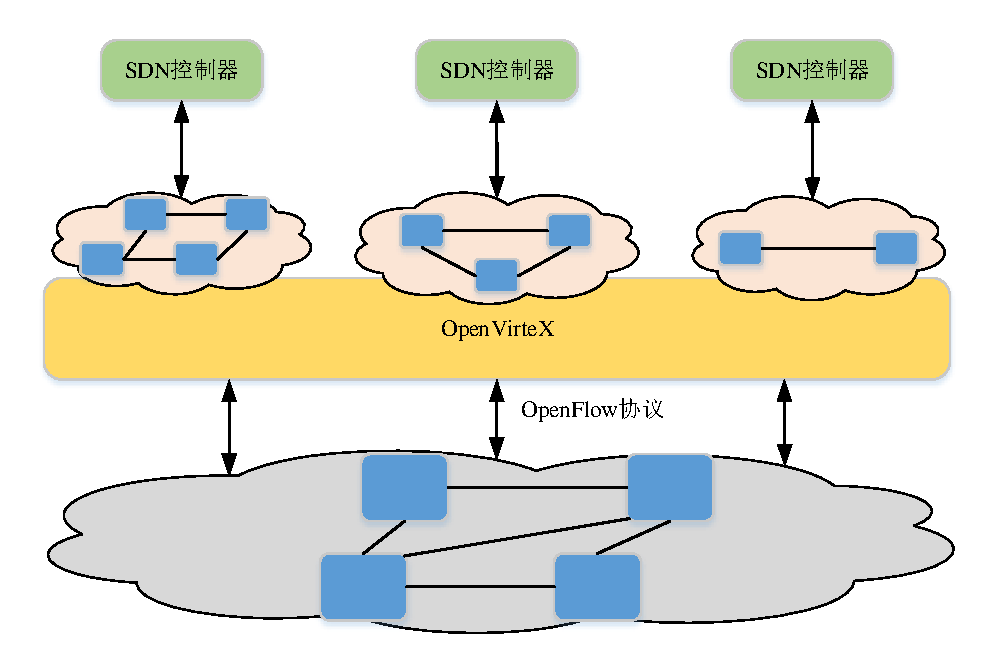
\includegraphics[width=0.7\textwidth]{logo/ovx}
  \caption{OVX网络虚拟化示意图}
  \label{fig:ovx}
\end{figure}

\section{OpenStack概述}

OpenStack是一个开源的云平台,主要为企业或厂商提供一种云服务的解决方案\cite{OpenStack-5}。OpenStack既可以直接被企业使用,在企业局域网内提供私有云服务;也可以被厂商使用,进行二次开发,给用户提供通过网络访问的公有云服务\cite{OpenStack-6}。

\subsection{OpenStack架构}
OpenStack\ Juno版本的构架由9个服务组成,分别是计算(Nova)、对象存储(Swift)、网络(Neutron)、镜像(Glance)、块存储(Cinder)、认证(Keystone)、编排(Heat)、监控(Ceilometer)、Web界面(Horizon)\cite{OpenStack-4}。各服务对应的组件及各组件之间的协同关系如图\ref{fig:openstack}所示。

\begin{figure}[!htb]
  \centering
  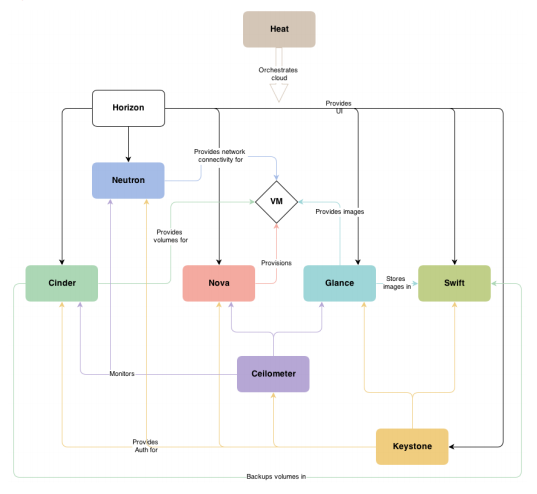
\includegraphics[width=0.7\textwidth]{logo/openstack}
  \caption{OpenStack概念架构图}
  \label{fig:openstack}
\end{figure}

主要组件的功能介绍如下\cite{OpenStack-3}。

\begin{enumerate}
\item Nova:计算服务,主要包括虚拟机的创建、调度、修改以及销毁等功能。nova-compute实现对虚拟机生命周期的管理,该服务运行于各计算节点;nova-api提供开发的API接口;nova-scheduler运行于控制节点,在创建虚拟机时,负责将虚拟机调度到某个计算节点进行虚拟机的创建。
\item Swift:对象存储,主要实现OpenStack中,数据对象的存储备份。在OpenStack云平台中,任何一个数据都可以看作是一个对象,通过swift-proxy服务进行数据的存取,每个数据对象的定位需要三个模块,分别为account、container和object。
\item Neutron:网络模块,该模块主要提供云平台中的各种网络服务,在云平台中提供服务的大致流程如下:首先进行网络和子网的创建,创建的网络用于挂载租户创建的虚拟机,在租户启动虚拟机时,创建的子网会为该虚拟机分配网络端口,而在虚拟机删除时,需要将虚拟机及其绑定的网络端口一并删除,在网络不需要时,删除网络资源。后续章节会对该模块做详细介绍。
\item Glance:镜像服务,该模块用于管理OpenStack提供的虚拟机镜像,在租户创建镜像时,Glance会将该镜像信息注册到数据库,在虚拟机创建时,选取相应的镜像资源,通过计算服务的调度,在服务器上基于该镜像实例化一个虚拟机。
\item Cinder:块存储,该模块主要为云平台提供块存储和备份功能,租户可以为自己的虚拟机添加块存储,在虚拟机启动后,可以像操作本地硬盘一样操作该块存储设备。
\item KeyStone:认证服务,主要实现用户、租户、角色等信息的认证,该服务提供认证相关的元数据,所有用户的请求操作,都需要经过Keystone模块进行身份认证,认证成功后方才进行相应请求的执行。
\item Heat:编排服务,主要为用户提供一套完整的业务部署平台,通过为用户提供服务模板,实现资源的自动化快速部署。
\item Ceilometer:监控服务,主要用于收集云平台运行状态信息,比如:内存使用率、CPU使用率、数据包传输速率、硬盘使用情况等。对于采集到的数据,Ceilometer提供给报警和计费模块使用。
\item Horizon:Web界面服务,Horizon是为用户开放的Web界面,现有模式下,大多数服务均可在界面实现相应的操作,虚拟机管理、镜像管理、块存储管理、对象存储管理、网络管理等均可在Web界面实现相应的操作。
\end{enumerate}
\subsection{Neutron模块详解}
本文研究的主要内容,涉及最多的是OpenStack的Neutron模块,故本节对Neutron模块做详细的介绍,方便大家对论文的理解。

Neutron组件基于软件定义的思想实现各种网络服务,通常情况下,Neutron中的网络模式主要包括GRE、VLAN、VXLAN,本文中选取GRE模式进行Neutron服务的搭建,GRE模式下的Neutron架构图如图\ref{fig:neutron}所示。

\begin{figure}[!htb]
  \centering
  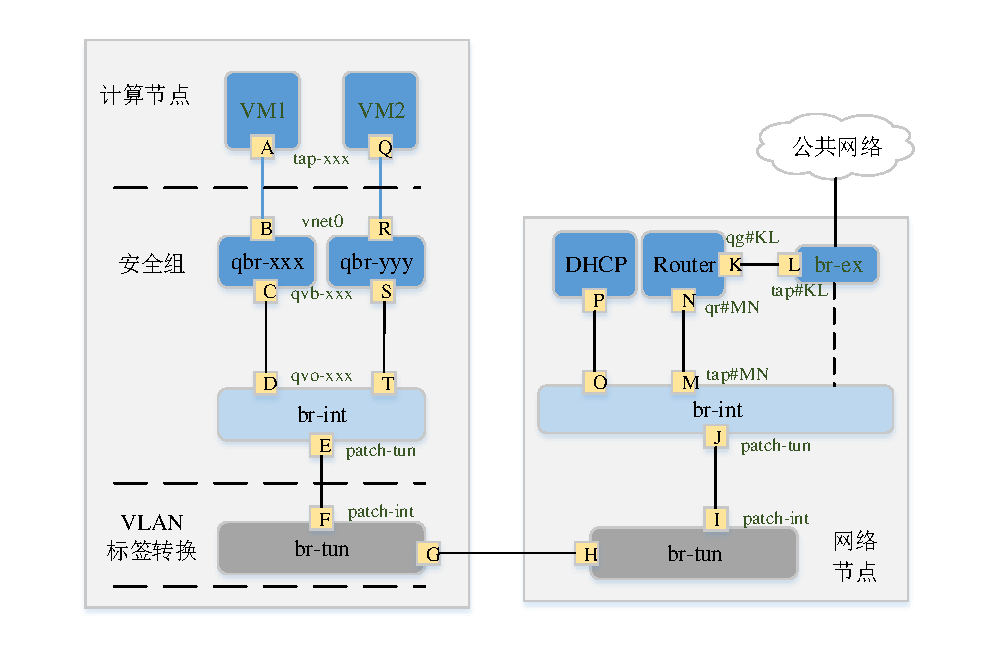
\includegraphics[width=0.7\textwidth]{logo/neutron}
  \caption{Neutron组件GRE模式架构图}
  \label{fig:neutron}
\end{figure}

在OpenStack中,网络节点部署和网络有关的所有服务,而在计算节点只需要提供适用于虚拟机的基本网络功能,包括安全组、隔离不同租户的虚拟机等服务,以GRE模式下的架构图为例,计算节点在qbr-xxx网桥上进行虚拟机安全组的配置,在网络节点上,Neutron组件配置有DHCP、Router服务,对于访问外网的数据包,全部经由br-ex发出。各网桥功能及具体服务如下所示。

\begin{enumerate}
\item qbr:由图\ref{fig:neutron}可以看出,虚拟机网卡挂载到物理服务器的一个TAP设备上面,由于OpenStack需要利用Linux的iptables为租户虚拟机提供安全组服务,而现阶段,OVS交换机并不支持应用iptables 规则的 Tap 设备,所以,TAP设备并没有直接连接至br-int网桥,而是通过qbr实现与br-int网桥的连接,为虚拟机提供安全组服务。

\item br-int:该网桥中仅包含一条流表——正常转发。如果同一服务器的同一租户的虚拟机(虚拟机具有相同的vlan标签)之间进行通信,只需通过br-int网桥即可。在网络节点上,br-int网桥通过挂载多个应用进程来提供多样化的网络服务,由于不同租户公共这些进程,相互之间的地址空间必然会存在冲突,因此每一项网络服务均需要运行在自己的网络命名空间中。
\item br-tun:该网桥主要实现对vlan 号和tunnel号的封装工作,当数据包从该服务器发出时,为该数据包封装tunnel号,而对于从外部服务器接收到的数据包,需要根据tunnel号为该数据包添加vlan标签。该网桥的整体转发逻辑如图\ref{fig:br-tun}所示。所有到达br-tun的网包,均交给Table0,如果该数据包来自gre端口,即从外部服务器发送至此,则交给Table2进一步处理;如果该数据包来自patch-int端口,即从服务器内部发出,目的主机位于服务器之外,则交给Table1进行下一步的处理,否则丢弃该包。Table2主要的作用是根tunnel号为数据包添加vlan号;Table10主要实现了反向规则的添加,Table20和Table21主要实现了vlan号向tunnel号的转换,两者的区别在于,Table20主要针对单播,而Table21主要针对多播/组播。

\begin{figure}[!htb]
  \centering
  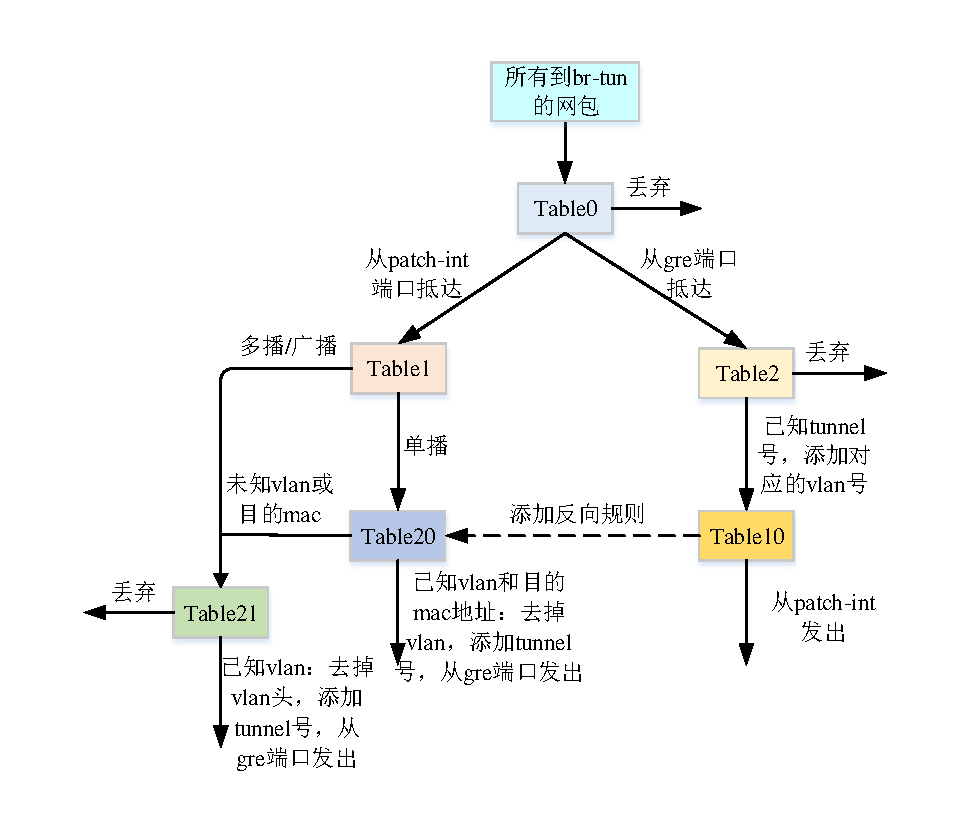
\includegraphics[width=0.7\textwidth]{logo/br-tun}
  \caption{br-tun网桥转发规则}
  \label{fig:br-tun}
\end{figure}

\item br-ex:虚拟机访问外网时,数据包均从br-ex发出,该网桥是虚拟机与外网通信的必经之路。
\item dhcp 服务:dhcp服务主要为租户虚拟机提供IP地址。该服务是通过 Linux内的dnsmasq 进程实现,该进程可以为用户提供dhcp、dns等网络服务。 
\item router服务:router服务主要为租户提供跨子网的通信功能,比如,云平台内部虚拟机访问外部网络,那么该数据包必须经过router进行地址转换,完成云平台虚拟机与外网的通信。现阶段router服务基于Linux的iptables实现,每个router服务都具有特有的网络命名空间,实现租户之间的隔离。

\end{enumerate}

\section{本章小结}
本章主要介绍了SDN、网络虚拟化及OpenStack的相关技术。重点介绍了OpenFlow协议,OpenFlow交换机的组成以及OpenFlow流表主要字段以及流表匹配过程。对于网络虚拟化技术,由于本文需要实现SDN模式下的网络虚拟化,所以仅对适用于本文的SDN模式下的网络虚拟化技术做了简单的概括。随后介绍了OpenStack的模块构成,而对于本文用到的Neutron模块,进行了详细的架构剖析。本文的系统架构,主要在以上各部分的基础上,进行集成开发。后续会对整体的系统架构做详细的介绍。